\documentclass[10pt,a4paper]{article}
\usepackage[margin=12mm]{geometry}
\usepackage{amsmath,amssymb,tikz,caption}
\usetikzlibrary{arrows.meta,positioning,calc,shapes.geometric}
\pagestyle{empty}
\begin{document}
\begin{center}
{\large\bfseries FRACMATH: numerical damage update}\\[4pt]
\end{center}
The diagram shows the default modified von Mises driver. The CPU Mazars, stress Rankine and smooth stress Rankine options replace this calculation while keeping the other operations. The modified von Mises driver used below is
\[
\mathcal E_{\mathrm{mvM}}(I_1,J_2)=
\frac{k-1}{2k(1-2\nu)}I_1+
\frac{1}{2k}\sqrt{\left(\frac{k-1}{1-2\nu}\right)^2I_1^2+
\frac{12k}{(1+\nu)^2}J_2},\qquad k=f_c/f_t.
\]
\noindent $E$ is Young's modulus; $\nu$ is Poisson's ratio; $f_t$ and $f_c$ are tensile and compressive strengths; $G_F$ is fracture energy per crack area. Engineering shear is $\gamma_{xy}$ and tensor shear is $\gamma_{xy}/2$. The diagram shows the Oliver-width implementation.\\[5pt]

\centering
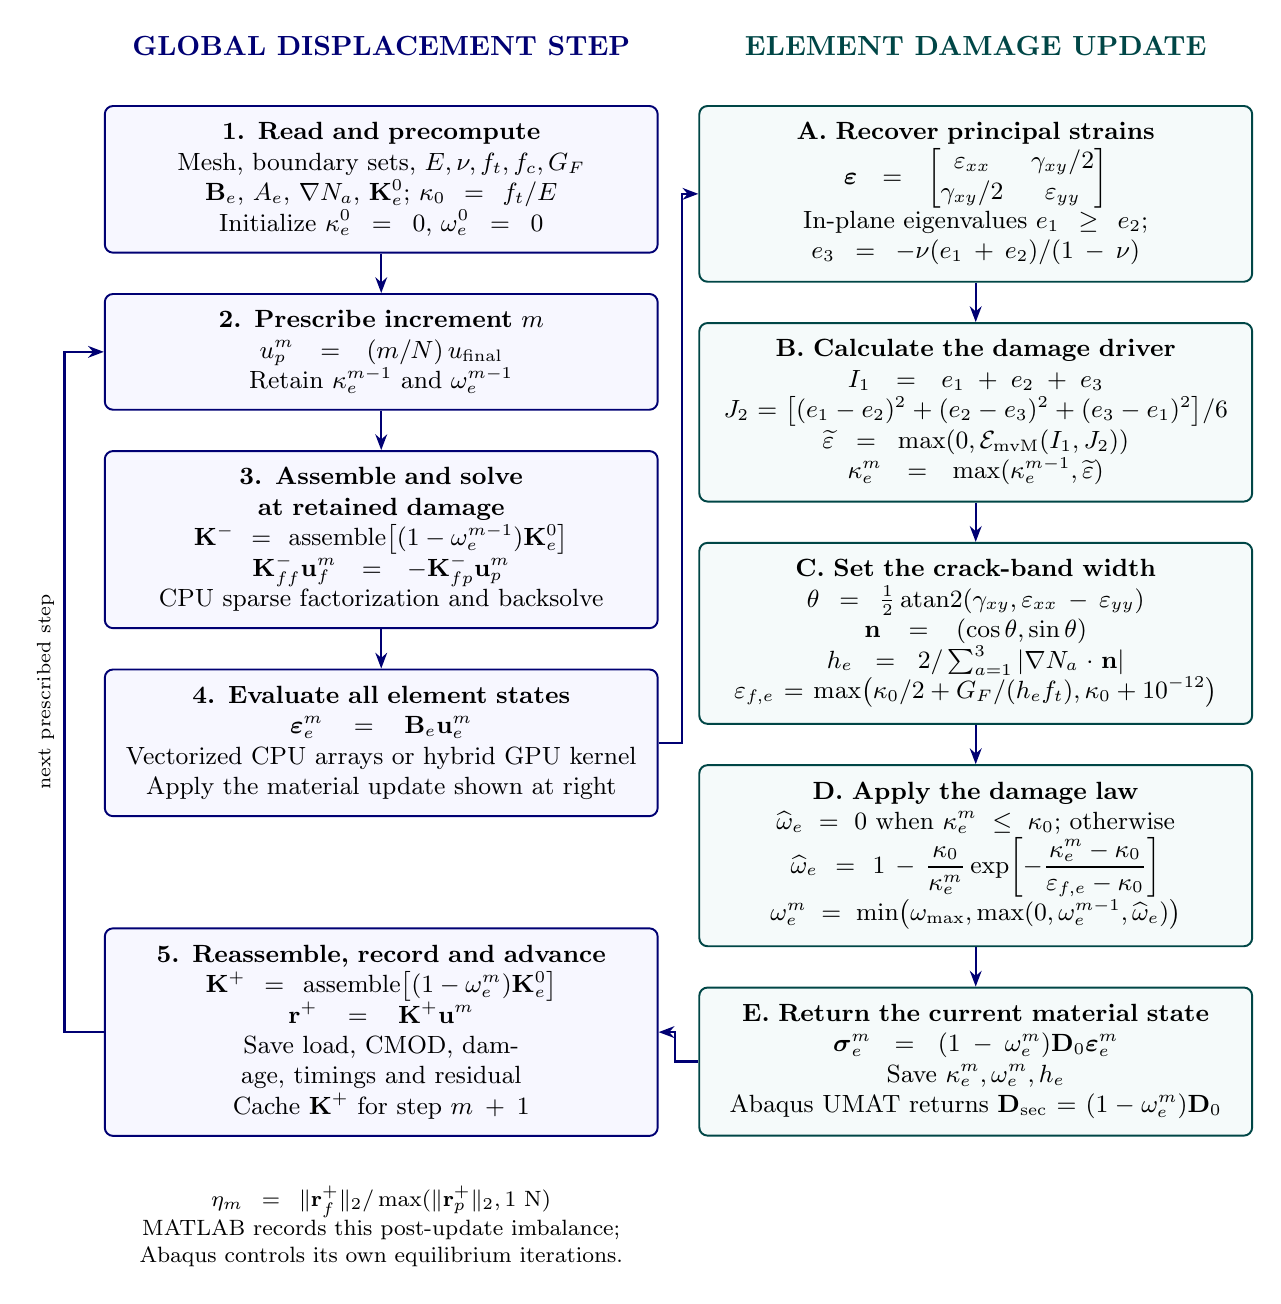
\begin{tikzpicture}[
  font=\small,
  process/.style={draw=blue!45!black,fill=blue!3,rounded corners=3pt,
    line width=0.7pt,text width=6.6cm,align=center,inner sep=6pt},
  material/.style={process,draw=teal!55!black,fill=teal!4},
  line/.style={-{Stealth[length=2mm]},line width=0.8pt,draw=blue!45!black},
  note/.style={font=\footnotesize,align=center,text width=6.6cm},
  node distance=5mm]
\node[font=\bfseries,text=blue!45!black] (globaltitle) at (0,0) {GLOBAL DISPLACEMENT STEP};
\node[font=\bfseries,text=teal!55!black] (localtitle) at (7.55,0) {ELEMENT DAMAGE UPDATE};
\node[process,below=5mm of globaltitle] (input) {\textbf{1. Read and precompute}\\
Mesh, boundary sets, $E,\nu,f_t,f_c,G_F$\\
$\mathbf B_e$, $A_e$, $\nabla N_a$, $\mathbf K_e^0$; $\kappa_0=f_t/E$\\
Initialize $\kappa_e^0=0$, $\omega_e^0=0$};
\node[process,below=of input] (load) {\textbf{2. Prescribe increment $m$}\\
$u_p^m=(m/N)\,u_{\mathrm{final}}$\\
Retain $\kappa_e^{m-1}$ and $\omega_e^{m-1}$};
\node[process,below=of load] (solve) {\textbf{3. Assemble and solve at retained damage}\\
$\mathbf K^-=\operatorname{assemble}\!\left[(1-\omega_e^{m-1})\mathbf K_e^0\right]$\\
$\mathbf K^-_{ff}\mathbf u_f^m=-\mathbf K^-_{fp}\mathbf u_p^m$\\
CPU sparse factorization and backsolve};
\node[process,below=of solve] (dispatch) {\textbf{4. Evaluate all element states}\\
$\boldsymbol\varepsilon_e^m=\mathbf B_e\mathbf u_e^m$\\
Vectorized CPU arrays or hybrid GPU kernel\\
Apply the material update shown at right};
\node[material,below=5mm of localtitle] (strain) {\textbf{A. Recover principal strains}\\
$\boldsymbol\varepsilon=\begin{bmatrix}\varepsilon_{xx}&\gamma_{xy}/2\\\gamma_{xy}/2&\varepsilon_{yy}\end{bmatrix}$\\
In-plane eigenvalues $e_1\geq e_2$;\\
$e_3=-\nu(e_1+e_2)/(1-\nu)$};
\node[material,below=of strain] (equivalent) {\textbf{B. Calculate the damage driver}\\
$I_1=e_1+e_2+e_3$\\
$J_2=\big[(e_1-e_2)^2+(e_2-e_3)^2+(e_3-e_1)^2\big]/6$\\
$\widetilde\varepsilon=\max(0,\mathcal E_{\mathrm{mvM}}(I_1,J_2))$\\
$\kappa_e^m=\max(\kappa_e^{m-1},\widetilde\varepsilon)$};
\node[material,below=of equivalent] (width) {\textbf{C. Set the crack-band width}\\
$\theta=\tfrac12\operatorname{atan2}(\gamma_{xy},\varepsilon_{xx}-\varepsilon_{yy})$\\
$\mathbf n=(\cos\theta,\sin\theta)$\\
$h_e=2/\sum_{a=1}^3|\nabla N_a\!\cdot\!\mathbf n|$\\
$\varepsilon_{f,e}=\max\!\left(\kappa_0/2+G_F/(h_e f_t),\kappa_0+10^{-12}\right)$};
\node[material,below=of width] (damage) {\textbf{D. Apply the damage law}\\
$\widehat\omega_e=0$ when $\kappa_e^m\leq\kappa_0$; otherwise\\
$\widehat\omega_e=1-\dfrac{\kappa_0}{\kappa_e^m}
\exp\!\left[-\dfrac{\kappa_e^m-\kappa_0}{\varepsilon_{f,e}-\kappa_0}\right]$\\
$\omega_e^m=\min\!\left(\omega_{\max},\max(0,\omega_e^{m-1},\widehat\omega_e)\right)$};
\node[material,below=of damage] (stress) {\textbf{E. Return the current material state}\\
$\boldsymbol\sigma_e^m=(1-\omega_e^m)\mathbf D_0\boldsymbol\varepsilon_e^m$\\
Save $\kappa_e^m,\omega_e^m,h_e$\\
Abaqus UMAT returns $\mathbf D_{\mathrm{sec}}=(1-\omega_e^m)\mathbf D_0$};
\node[process,below=14mm of dispatch] (reaction) {\textbf{5. Reassemble, record and advance}\\
$\mathbf K^+=\operatorname{assemble}\!\left[(1-\omega_e^m)\mathbf K_e^0\right]$\\
$\mathbf r^+=\mathbf K^+\mathbf u^m$\\
Save load, CMOD, damage, timings and residual\\
Cache $\mathbf K^+$ for step $m+1$};
\node[note,below=5mm of reaction] (residual) {$\eta_m=\|\mathbf r_f^+\|_2/\max(\|\mathbf r_p^+\|_2,1~\mathrm N)$\\
MATLAB records this post-update imbalance;\\
Abaqus controls its own equilibrium iterations.};
\draw[line] (input)--(load);
\draw[line] (load)--(solve);
\draw[line] (solve)--(dispatch);
\draw[line] (strain)--(equivalent);
\draw[line] (equivalent)--(width);
\draw[line] (width)--(damage);
\draw[line] (damage)--(stress);
\draw[line] (dispatch.east)--++(3mm,0) |- (strain.west);
\draw[line] (stress.west)--++(-3mm,0) |- (reaction.east);
\draw[line] (reaction.west)--++(-5mm,0) |- node[pos=0.25,rotate=90,above,font=\scriptsize] {next prescribed step} (load.west);
\end{tikzpicture}
\captionof{figure}{Step-by-step 2D damage calculation and sequential MATLAB implementation, drawn directly in LaTeX. Subscripts $e,f,p$ denote element, free and prescribed degrees of freedom; $m$ is the increment index and $N$ its prescribed total. $\mathbf D_0$ and $\mathbf K_e^0$ are elastic material and element matrices; $\mathbf B_e$ maps element displacements to strain. $\widehat\omega_e$ is the trial damage and $\omega_{\max}=1-10^{-12}$ is the 2D damage cap. The UMAT uses the same material equations but Abaqus supplies trial strains and controls nonlinear equilibrium; the global MATLAB path is not an Abaqus iteration algorithm.}
\label{fig:implementation}


\end{document}
